\section{Experiment: Toy Problem}

\begin{frame}{Problem Definition}

phenotype: $\vec{x} = \{l_1, l_2, \dots, l_{100} \}$
\begin{itemize}
\item 100-legged ``table''
\end{itemize}

fitness: $−\sigma(\vec{x})$
\begin{itemize}
\item best fitness = level table
\end{itemize}

rugged fitness landscape:
any level table is a local fitness peak

\end{frame}

\begin{frame}{Problem Definition}

response to selection experiments

fitness:
$−\sigma(⃗\vec{x}) − |\mu(\vec{x})/10 |$


intuition:
level-ness still essential, but short tables tend to be favored

\end{frame}

\begin{frame}{G-P Map Implementations}

\begin{columns}
\begin{column}{0.5\textwidth}
100-to-100 fully-connected layer
graphic: TODO
\begin{itemize}
\item intuition: averaging
\end{itemize}
\end{column}
\begin{column}{0.5\textwidth}
graphic: TODO
intuition: single underlying value
\end{column}
\end{columns}

\end{frame}

\begin{frame}{Experiment}

\begin{itemize}
\item make training data: 250 independent populations of 300 individuals evolved with direct encoding
\item train autoencoder
\item reviewer comment on param settings %TODO
\end{itemize}

\end{frame}


\begin{frame}{Result: Response to Selective Pressure}

\begin{figure}
  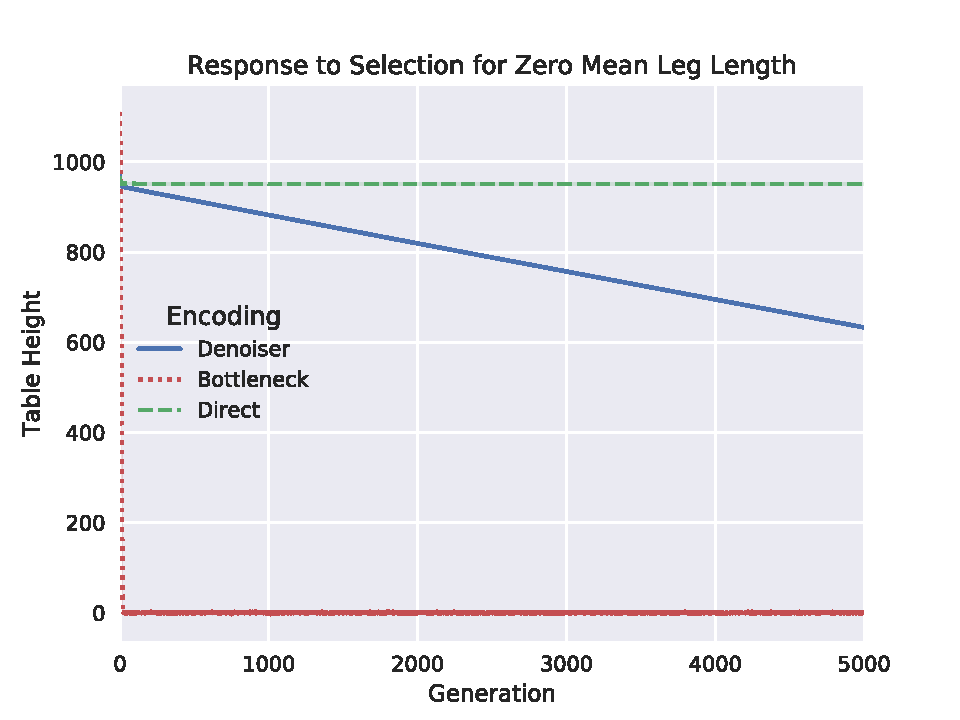
\includegraphics[width=0.85\linewidth]{img/results/zero_leg_selection}
  \caption{
    Response to short-table selection pressure under different genotype-phenotype maps.
    Bootstrapped 95\% confidence intervals are shaded along each curve.
  }\label{fig:select_response}
\end{figure}


TODO: per-stie mutation rate?!?

\end{frame}
